% ===============================================================
%  جلسه هفدهم
% ===============================================================
\chapter{مثال‌های معروف از $g(X,Y)$، آماره‌های ترتیبی و قضیه حد مرکزی}

\section{مثال‌های معروف از $g(X,Y)$}

\subsection{توزیع کای‌دو \lr{($\chi^2(k)$ یا Chi-Square)} با $k$ درجه آزادی}

\begin{definition}[توزیع کای‌دو]
فرض کنید $X_1,X_2,\ldots,X_k$ متغیرهای تصادفی گاوسی \textbf{مستقل} و \textbf{استاندارد} (دارای میانگین صفر و واریانس ۱) باشند. در این صورت متغیر تصادفی
\[
Z=\sum_{i=1}^{k}X_i^2
\]
را دارای توزیع $\chi^2(k)$ می‌نامیم.
\end{definition}
کاربرد: مجموع مربعات خطاهای مستقل گاوسی (مثلاً توان نویز در $k$ نمونه، یا آماره‌های آزمون فرض در آمار).

\begin{example}[چگالی $\chi^2(2)$]
\textcolor{red!70!black}{سؤال:} تابع چگالی احتمال $\chi^2(2)$ را بیابید.
\begin{solution}
ابتدا تابع توزیع انباشته را به دست می‌آوریم. با $Z=X^2+Y^2$ و $f_{XY}=\frac{1}{2\pi}e^{-(x^2+y^2)/2}$ (استقلال)، ناحیه $\{Z\le z\}$ یک دایره به شعاع $\sqrt z$ است:
\[
F_Z(z)=\iint_{x^2+y^2\le z}\frac{1}{2\pi}e^{-\frac{x^2+y^2}{2}}\dd x\dd y=\frac{1}{2\pi}\int_0^{2\pi}\!\!\int_0^{\sqrt z}e^{-r^2/2}\,r\dd r\dd\theta .
\]
همان‌طور که مشاهده شد، با تغییر مختصات از \textbf{دکارتی} به \textbf{قطبی} ($x=r\cos\theta$، $y=r\sin\theta$، $\dd x\dd y=r\dd r\dd\theta$)، فرم دلخواه پیش‌تر اشاره شده برای توزیع انباشته حاصل می‌شود. با مشتق‌گیری نسبت به $z$ از $F_Z(z)$ (قاعده لایبنیتس روی حد بالای $\sqrt z$)، چگالی احتمال $\chi^2(2)$ به دست خواهد آمد:
\[
f_Z(z)=\frac{1}{2\pi}\int_0^{2\pi}\frac{\partial\sqrt z}{\partial z}\,e^{-(\sqrt z)^2/2}\sqrt z\dd\theta=\frac{1}{2\pi}\cdot2\pi\cdot\frac{1}{2\sqrt z}e^{-z/2}\sqrt z=\frac{e^{-z/2}}{2}u(z).
\]
(مستقیم‌تر: $F_Z(z)=\int_0^{\sqrt z}e^{-r^2/2}r\dd r=1-e^{-z/2}$.)
\end{solution}
\end{example}

\begin{note}
\notetitle در حالت خاص $k=2$، توزیع $\chi^2(k)$ برابر با یک توزیع \textbf{نمایی} (با پارامتر $\lambda=\frac12$) خواهد شد.
\end{note}

\begin{question}[سعی کنید ضابطه $\chi^2(k)$ را برای $k>2$ در خانه به دست آورید.]
\begin{answer}
\textbf{روش \lr{MGF}:} برای $X\sim\mathcal N(0,1)$:
\[
M_{X^2}(t)=\E e^{tX^2}=\int\frac{1}{\sqrt{2\pi}}e^{-\frac{(1-2t)x^2}{2}}\dd x=(1-2t)^{-1/2},\qquad t<\tfrac12 .
\]
با استقلال، $M_Z(t)=(1-2t)^{-k/2}$. از طرفی چگالی $g(z)=\frac{z^{a-1}e^{-z/2}}{2^a\Gamma(a)}$ (توزیع گاما با شکل $a$ و مقیاس ۲) دارای \lr{MGF} برابر $(1-2t)^{-a}$ است (با تغییر متغیر $w=(1-2t)z/2$ و تعریف تابع گاما). پس با $a=k/2$ و یکتایی:
\[
\boxed{\ f_{\chi^2(k)}(z)=\frac{1}{2^{k/2}\Gamma(k/2)}\,z^{\frac k2-1}e^{-z/2}\,u(z)\ }
\]
بررسی: $k=2$: $\frac{1}{2\Gamma(1)}e^{-z/2}=\frac12e^{-z/2}$ \checkmark. $k=1$: $\frac{1}{\sqrt2\Gamma(1/2)}z^{-1/2}e^{-z/2}=\frac{1}{\sqrt{2\pi z}}e^{-z/2}$ که با نتیجه جلسه یازدهم برای $X^2$ مطابقت دارد \checkmark. همچنین $\E Z=k$ و $\Var Z=2k$.
\end{answer}
\end{question}

\begin{center}
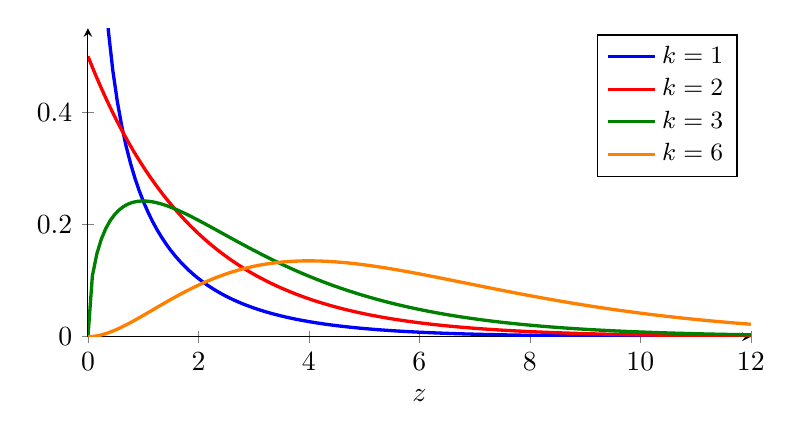
\begin{tikzpicture}
\begin{axis}[width=10cm,height=5.5cm,axis lines=left,xmin=0,xmax=12,ymin=0,ymax=0.55,xlabel={$z$},samples=150,legend style={font=\small}]
\addplot[blue,very thick,domain=0.05:12] {exp(-x/2)/sqrt(2*pi*x)}; \addlegendentry{$k=1$}
\addplot[red,very thick,domain=0:12] {exp(-x/2)/2}; \addlegendentry{$k=2$}
\addplot[green!50!black,very thick,domain=0:12] {sqrt(x)*exp(-x/2)/(2^(1.5)*0.886227)}; \addlegendentry{$k=3$}
\addplot[orange,very thick,domain=0:12] {x^2*exp(-x/2)/(8*2)}; \addlegendentry{$k=6$}
\end{axis}
\end{tikzpicture}
\end{center}

\subsection{توزیع رایلی و توزیع نسبت (اثبات در کتاب)}

\begin{theorem}[رایلی]
فرض کنید که متغیرهای تصادفی $X,Y$ گاوسی $\mathcal N(0,\sigma^2)$ و مستقل باشند. تعریف می‌کنیم $Z=\sqrt{X^2+Y^2}$. آنگاه $Z$ توزیع رایلی (\lr{Rayleigh}) دارد:
\[
f_Z(z)=\frac{z}{\sigma^2}e^{-z^2/(2\sigma^2)}u(z).
\]
\end{theorem}
\begin{proof}
مانند مثال $\chi^2(2)$ با مختصات قطبی:
$F_Z(z)=\Prob(X^2+Y^2\le z^2)=\frac{1}{2\pi\sigma^2}\int_0^{2\pi}\!\int_0^ze^{-r^2/2\sigma^2}r\dd r\dd\theta=1-e^{-z^2/2\sigma^2}$ برای $z\ge0$. با مشتق‌گیری حکم ثابت می‌شود. (معادلاً $Z^2/\sigma^2\sim\chi^2(2)$.)
\end{proof}
کاربرد: دامنه (پوش) سیگنال در کانال‌های بی‌سیم با محوشدگی، که مؤلفه‌های هم‌فاز و متعامد آن گاوسی مستقل‌اند.

\begin{theorem}[نسبت دو گاوسی ← کوشی]
فرض کنید که متغیرهای تصادفی $X,Y$ مشترکاً گاوسی با میانگین‌های صفر، واریانس‌های $\sigma_1^2$ و $\sigma_2^2$، و ضریب همبستگی $r$ باشند. تعریف می‌کنیم $Z=X/Y$. آنگاه $Z$ توزیع کوشی (\lr{Cauchy}) حول مقدار $\frac{r\sigma_1}{\sigma_2}$ دارد:
\[
f_Z(z)=\frac{\gamma/\pi}{(z-x_0)^2+\gamma^2},\qquad x_0=\frac{r\sigma_1}{\sigma_2},\quad\gamma=\frac{\sigma_1}{\sigma_2}\sqrt{1-r^2}.
\]
\end{theorem}
\begin{proof}[طرح اثبات]
برای نسبت، $F_Z(z)=\Prob(X\le zY,\ Y>0)+\Prob(X\ge zY,\ Y<0)$ و با مشتق‌گیری به فرمول کلی زیر می‌رسیم:
\[
f_Z(z)=\int_{-\infty}^{\infty}|y|\,f_{XY}(zy,\ y)\dd y .
\]
با جایگذاری چگالی مشترکاً گاوسی، انتگرالده به شکل $|y|e^{-Ay^2}$ با $A=\frac{1}{2(1-r^2)}\big(\frac{z^2}{\sigma_1^2}-\frac{2rz}{\sigma_1\sigma_2}+\frac{1}{\sigma_2^2}\big)$ است و $\int|y|e^{-Ay^2}\dd y=\frac1A$. پس
$f_Z(z)=\frac{1}{2\pi\sigma_1\sigma_2\sqrt{1-r^2}}\cdot\frac{1}{A}$ و با ساده‌سازی (تکمیل مربع در مخرج) به فرم کوشی بالا می‌رسیم. در حالت خاص $r=0$ و $\sigma_1=\sigma_2$: نسبت دو گاوسی استاندارد مستقل، کوشی استاندارد است.
\end{proof}

\section{آماره‌های ترتیبی \lr{(min, max و \ldots)}}

متغیرهای تصادفی $X_1,X_2,\ldots,X_n$ را به صورت \lr{i.i.d.} با توزیع انباشته $F_X$ و تابع چگالی احتمال $f_X$ در نظر بگیرید. متغیرهای تصادفی جدید $L,U$ را تعریف می‌کنیم:
\[
L=\min(X_1,X_2,\ldots,X_n),\qquad U=\max(X_1,X_2,\ldots,X_n).
\]
توابع چگالی احتمال $f_U$ و $f_L$ چگونه به دست خواهند آمد؟

\subsection{تابع چگالی احتمال کمینه}
در مورد توزیع $L$ مطابق با زیر عمل خواهیم کرد: فرض کنید $h\to0^+$. در این صورت داریم (با نماد $X_{-i}>\ell$ یعنی «همه $X_j$ها به جز $X_i$ از $\ell$ بزرگ‌ترند»):
\[
\begin{aligned}
f_L(\ell)\,h&=\Prob(\ell\le L\le\ell+h)=\Prob\Big(\bigcup_{i=1}^{n}\big[\ell\le X_i\le\ell+h\ ,\ X_{-i}>\ell\big]\Big)\\
&=n\,\Prob\big(\ell\le X_1\le\ell+h\ ,\ X_{-1}>\ell\big).
\end{aligned}
\]
(رخدادهای اجتماع، تا مرتبه $o(h)$، ناسازگارند ــ احتمال اینکه دو متغیر هم‌زمان در بازه‌ای به طول $h$ بیفتند از مرتبه $h^2$ است ــ و به دلیل تقارن \lr{i.i.d.} همه احتمال برابر دارند.) با توجه به تعریف توابع توزیع انباشته و چگالی احتمال (یعنی $F_X$ و $f_X$) و استقلال، می‌توان نوشت:
\[
\boxed{\ f_L(\ell)=n\,f_X(\ell)\big(1-F_X(\ell)\big)^{n-1}\ }
\]

\subsection{تابع چگالی احتمال بیشینه}
مشابه با قبل:
\[
\begin{aligned}
f_U(u)\,h&=\Prob(u\le U\le u+h)=\Prob\Big(\bigcup_{i=1}^{n}\big[u\le X_i\le u+h\ ,\ X_{-i}\le u\big]\Big)\\
&=n\,\Prob\big(u\le X_1\le u+h\ ,\ X_{-1}\le u\big),
\end{aligned}
\]
\[
\boxed{\ f_U(u)=n\,f_X(u)\,F_X^{n-1}(u)\ }
\]

\begin{note}
\notetitle \textbf{روش جایگزین (با \lr{CDF}):} $U\le u$ اگر و تنها اگر \emph{همه} $X_i\le u$؛ پس $F_U(u)=F_X(u)^n$. و $L>\ell$ اگر و تنها اگر همه $X_i>\ell$؛ پس $F_L(\ell)=1-(1-F_X(\ell))^n$. مشتق‌گیری همان فرمول‌های بالا را می‌دهد.
\end{note}

\begin{example}[بزرگ‌ترین و کوچک‌ترین از $n$ یکنواخت]
برای $X_i\sim\mathcal U(0,1)$ \lr{i.i.d.}: $f_U(u)=nu^{n-1}$ و $f_L(\ell)=n(1-\ell)^{n-1}$ روی $[0,1]$. پس $\E U=\frac{n}{n+1}$ و $\E L=\frac{1}{n+1}$: $n$ نقطه تصادفی، بازه $[0,1]$ را به طور متوسط به $n+1$ قطعه مساوی تقسیم می‌کنند.
\end{example}

\subsection{در خانه حل کنید}

\begin{question}[اگر $X_1,\ldots,X_n$ مستقل باشند اما هم‌توزیع نباشند (فرض \lr{i.i.d.} برقرار نباشد)، روابط $f_U$ و $f_L$ چه تغییری می‌کنند؟]
\begin{answer}
با همان استدلال \lr{CDF} و استقلال:
\[
F_U(u)=\prod_{i=1}^nF_i(u),\qquad f_U(u)=\sum_{i=1}^nf_i(u)\prod_{j\ne i}F_j(u),
\]
\[
F_L(\ell)=1-\prod_{i=1}^n\big(1-F_i(\ell)\big),\qquad f_L(\ell)=\sum_{i=1}^nf_i(\ell)\prod_{j\ne i}\big(1-F_j(\ell)\big).
\]
(ضریب $n$ به جمع روی $i$ تبدیل می‌شود، زیرا دیگر همه جملات برابر نیستند.) مثال: کمینه نمایی‌های مستقل با نرخ‌های $\lambda_i$، نمایی با نرخ $\sum\lambda_i$ است.
\end{answer}
\end{question}

\begin{question}[اگر متغیرها نه مستقل و نه هم‌توزیع باشند (حالت کلی) چطور؟]
\begin{answer}
باید از توزیع مشترک استفاده کرد:
\[
F_U(u)=\Prob(X_1\le u,\ldots,X_n\le u)=F_{X_1,\ldots,X_n}(u,u,\ldots,u),
\]
\[
F_L(\ell)=1-\Prob(X_1>\ell,\ldots,X_n>\ell),
\]
که احتمال دوم با شمول و عدم شمول بر حسب \lr{CDF} مشترک قابل بیان است (مانند $\Prob(X>x,Y>y)$ در جلسه سیزدهم). چگالی‌ها با مشتق‌گیری به دست می‌آیند.
\end{answer}
\end{question}

\begin{question}[اگر به جای کمینه یا بیشینه، به دنبال سایر آماره‌های ترتیبی باشیم چطور؟ مثلاً توزیع دومین مقدار بزرگ؟ یا توزیع یکی‌مانده‌به‌کوچک‌ترین؟]
\begin{answer}
اگر $X_{(k)}$ را $k$امین کوچک‌ترین مقدار (در حالت \lr{i.i.d.}) بگیریم، برای اینکه $X_{(k)}\in[x,x+h]$ باشد باید: یکی از متغیرها در $[x,x+h]$، دقیقاً $k-1$ تا کمتر از $x$ و $n-k$ تا بیشتر از $x$ باشند. تعداد راه‌های تخصیص (توزیع چندجمله‌ای!) برابر $\frac{n!}{(k-1)!\,1!\,(n-k)!}$ است:
\[
\boxed{\ f_{X_{(k)}}(x)=\frac{n!}{(k-1)!\,(n-k)!}\,F_X(x)^{k-1}\big(1-F_X(x)\big)^{n-k}f_X(x)\ }
\]
$k=1$ کمینه و $k=n$ بیشینه را می‌دهد. «دومین مقدار بزرگ» یعنی $k=n-1$: $f(x)=n(n-1)F^{n-2}(1-F)f$. «یکی‌مانده‌به‌کوچک‌ترین» یعنی $k=2$: $f(x)=n(n-1)F(1-F)^{n-2}f$. برای یکنواخت، $X_{(k)}\sim\mathrm{Beta}(k,n-k+1)$ با میانگین $\frac{k}{n+1}$.
\end{answer}
\end{question}

\section{قضیه حد مرکزی \lr{(Central Limit Theorem)}}

\subsection{تعاریف}
در تمامی این بخش، فرض کنید که دنباله متناهی متغیرهای تصادفی $X_1,X_2,\ldots,X_n$ به صورت \lr{i.i.d.} توزیع شده و دارای تابع چگالی احتمال $f_X(\cdot)$ هستند. فرض کنید میانگین و واریانس این توزیع وجود داشته و به ترتیب برابر با $\mu$ و $\sigma^2$ باشند. متغیرهای تصادفی جدید $\bar X_n$ و $Z_n$ را مطابق با زیر تعریف می‌کنیم:
\[
\bar X_n=\frac{X_1+X_2+\cdots+X_n}{n},\qquad
Z_n=\frac{\sum_i(X_i-\mu)}{\sqrt n}=\sum_{i=1}^{n}\frac{X_i-\mu}{\sqrt n}.
\]
هدف، بررسی توزیع‌های حدی این دو متغیر در حالت $n\to\infty$ است.

\subsection{مرور قانون اعداد بزرگ}
در مورد متغیر تصادفی $\bar X_n$ (میانگین نمونه‌ای یا \lr{sample mean}) پیش‌تر مفصلاً بحث شد:
\begin{itemize}
\item این متغیر تصادفی دارای میانگین $\mu$ است.
\item همچنین، به دلیل فرض \lr{i.i.d.} واریانس آن از طریق رابطه زیر محاسبه می‌شود:
\[
\Var(\bar X_n)=\sum_i\Var\Big(\frac{X_i}{n}\Big)=\sum_i\frac{\sigma^2}{n^2}=\frac{\sigma^2}{n}.
\]
\item لذا واریانس در حد $n\to\infty$ برابر صفر شده، و متغیر تصادفی $\bar X_n$ در حد به مقدار یقینی $\mu$ میل می‌کند.
\end{itemize}

\subsection{ویژگی‌های $Z_n$}
در مورد متغیر تصادفی $Z_n$ (که انحراف $\bar X_n$ از $\mu$ را با ضریب $\sqrt n$ «بزرگ‌نمایی» می‌کند: $Z_n=\sqrt n(\bar X_n-\mu)$):
\begin{itemize}
\item این متغیر تصادفی دارای میانگین $0$ است:
\[
\E(Z_n)=\sum_i\Big(\frac{\E X_i-\mu}{n^{1/2}}\Big)=0 .
\]
\item به دلیل فرض \lr{i.i.d.}، واریانس $Z_n$ برابر با $\sigma^2$ خواهد بود:
\[
\Var(Z_n)=\sum_i\Var\Big(\frac{X_i-\mu}{n^{1/2}}\Big)=\sum_i\frac{\sigma^2}{n}=\sigma^2 .
\]
\end{itemize}
پس میانگین و واریانس $Z_n$ با $n$ تغییر نمی‌کنند. \textbf{اما توزیع $Z_n$ با افزایش $n$ به چه توزیعی میل خواهد کرد؟}

\subsection{محاسبه توزیع حدی $Z_n$}
فرض کنید داشته باشیم $X\sim f_X(x)$. متغیر تصادفی $X_c\triangleq X-\mu$ را به صورت نسخه مرکزی (یا \lr{zero-centered}) از $X$ تعریف می‌کنیم. همچنین، فرض کنید که تابع \lr{MGF} متناظر با $X_c$، $M_{X_c}(t)$ باشد. می‌توان به راحتی دید که:
\[
M_{(X_cn^{-1/2})}(t)=\E\big[e^{tX_c/\sqrt n}\big]=M_{X_c}\Big(\frac{t}{\sqrt n}\Big).
\]
به دلیل فرض \lr{i.i.d.}، و با توجه به خاصیت مطرح شده برای تابع \lr{MGF} جمع (جلسه یازدهم)، می‌توان نوشت:
\[
\boxed{\ M_{Z_n}(t)=\prod_{i=1}^{n}M_{X_c}\big(n^{-1/2}t\big)=M_{X_c}^n\big(n^{-1/2}t\big)\ }
\]
همچنین، حقایق زیر را در مورد تابع $M(\cdot)$ می‌دانیم:
\[
M_{X_c}(0)=1,\qquad M'_{X_c}(0)=\E[X_c]=0,\qquad M''_{X_c}(0)=\E[X_c^2]=\sigma^2 .
\]
در نتیجه (\textcolor{red!70!black}{با فرض همگرایی سری تیلور})، می‌توان دید برای $|t|\ll1$ داریم:
\[
M_{X_c}(t)=M_{X_c}(0)+M'_{X_c}(0)t+\tfrac12M''_{X_c}(0)t^2+O(t^3)=1+\tfrac12\sigma^2t^2+O(t^3).
\]
برای $M_{Z_n}(t)$ خواهیم داشت (با قرار دادن $t/\sqrt n$ به جای $t$؛ برای $t$ ثابت و $n$ بزرگ، $t/\sqrt n$ کوچک است):
\[
M_{Z_n}(t)=M_{X_c}^n\big(n^{-1/2}t\big)=\Big(1+\frac{\sigma^2t^2}{2n}+O\big(n^{-3/2}\big)\Big)^n ,
\]
و در حالت حدی، با استفاده از حد معروف $\lim_{n\to\infty}(1+\frac{a}{n}+o(\frac1n))^n=e^a$، می‌توان نوشت:
\[
\boxed{\ \lim_{n\to\infty}M_{Z_n}(t)=\lim_{n\to\infty}\Big(1+\frac{\sigma^2t^2}{2n}+O\big(n^{-3/2}\big)\Big)^n=\exp\Big(\frac12\sigma^2t^2\Big)\ }
\]

\subsection{توزیع حدی $Z_n$ در $n\to\infty$}
در نهایت، رابطه حدی زیر حاصل شد:
\[
\lim_{n\to\infty}M_{Z_n}(t)=e^{\frac{\sigma^2t^2}{2}},
\]
که بیانگر تابع مولد گشتاور (و به طور معادل، تابع مشخصه) یک توزیع گاوسی با میانگین صفر و واریانس $\sigma^2$ است. به عبارت دیگر، متغیر تصادفی $\lim_{n\to\infty}Z_n$ رفتار یک \textcolor{red!70!black}{\textbf{متغیر تصادفی گاوسی}} با توزیع $\mathcal N(0,\sigma^2)$ را دارد.

\begin{theorem}[قضیه حد مرکزی]
اگر $X_1,X_2,\ldots$ \lr{i.i.d.} با میانگین $\mu$ و واریانس متناهی $\sigma^2$ باشند، آنگاه برای هر $z$:
\[
\lim_{n\to\infty}\Prob\Big(\frac{\sum_{i=1}^n(X_i-\mu)}{\sigma\sqrt n}\le z\Big)=\Phi(z).
\]
\end{theorem}

\begin{note}
\notetitle \textbf{شگفتی قضیه:} توزیع اولیه $X_i$ هر چه باشد (یکنواخت، نمایی، برنولی، \ldots)، مجموع تعداد زیادی از آن‌ها تقریباً گاوسی است. این توضیح می‌دهد که چرا توزیع گاوسی این‌قدر در طبیعت ظاهر می‌شود: بسیاری از کمیت‌ها (خطای اندازه‌گیری، نویز حرارتی، قد انسان) حاصل جمع تعداد زیادی اثر کوچک و تقریباً مستقل‌اند. \textbf{کاربرد عملی:} $\sum_{i=1}^nX_i\approx\mathcal N(n\mu,n\sigma^2)$ و $\bar X_n\approx\mathcal N(\mu,\frac{\sigma^2}{n})$ برای $n$ بزرگ.
\end{note}

\subsection{چند مثال}
شکل‌های زیر توزیع $Z_n$ را برای $n=1,2,3$ و $n$ بزرگ نشان می‌دهند:

\textbf{توزیع پایه یکنواخت:}
\begin{center}
\foreach \n/\t in {1/{n=1},2/{n=2},3/{n=3},30/{n=30}}{%
\begin{tikzpicture}
\begin{axis}[width=4.6cm,height=4cm,axis lines=left,xmin=-1.2,xmax=1.2,ymin=0,ymax=1.6,xtick=\empty,ytick=\empty,title={$\t$}]
\addplot[black,thick] table[x=z,y=p]{data/ih\n.dat};
\end{axis}
\end{tikzpicture}}
\end{center}
(برای $n=2$ مثلثی (جلسه قبل)، برای $n=3$ از سه قطعه سهمی تشکیل شده و هم‌اکنون بسیار شبیه گاوسی است.)

\textbf{توزیع پایه برنولی} (با $p=0.3$):
\begin{center}
\foreach \n/\t in {1/{n=1},2/{n=2},3/{n=3},100/{n=100}}{%
\begin{tikzpicture}
\begin{axis}[width=4.6cm,height=4cm,axis lines=left,ymin=0,xtick=\empty,ytick=\empty,title={$\t$}]
\addplot+[ycomb,black,thick,mark=none] table[x=z,y=p]{data/bs\n.dat};
\end{axis}
\end{tikzpicture}}
\end{center}

\textbf{توزیع پایه گاوسی:} ؟

\begin{question}[اگر توزیع پایه خودش گاوسی باشد، توزیع $Z_n$ چیست؟]
\begin{answer}
طبق جلسه قبل، جمع گاوسی‌های مستقل، دقیقاً گاوسی است: $\sum(X_i-\mu)\sim\mathcal N(0,n\sigma^2)$ و $Z_n\sim\mathcal N(0,\sigma^2)$ \emph{برای هر $n$} ــ نه فقط در حد. توزیع گاوسی «نقطه ثابت» قضیه حد مرکزی است.
\end{answer}
\end{question}

\subsection{تفسیر همگرایی در قضیه حد مرکزی \lr{(CLT)}}
با توجه به مثال‌هایی که در بالا دیده شد:
\begin{itemize}
\item در صورتی که تابع توزیع پایه، برای مثال، \textbf{یکنواخت} انتخاب شود، تابع چگالی احتمال (\lr{PDF}) $Z_n$ به صورت نقطه به نقطه به $\mathcal N(0,\sigma^2)$ همگرا خواهد شد.
\item اما در صورتی که تابع توزیع پایه، برای مثال، \textbf{برنولی} انتخاب شود، چگالی احتمال $Z_n$ همواره به صورت یک رشته ضربه (دلتای دیراک) باقی خواهد ماند و در عمل به هیچ تابعی همگرا نمی‌شود.
\end{itemize}
لذا همگرایی $Z_n$ به یک متغیر تصادفی گاوسی مانند $Z^*\sim\mathcal N(0,\sigma^2)$ از حیث \textcolor{blue!60!black}{تابع چگالی احتمال} \textcolor{red!70!black}{نیست}.

\begin{question}[وقتی می‌گوییم متغیر تصادفی $Z_n$ به متغیر تصادفی $Z^*$ همگرا خواهد شد، منظور از همگرایی چیست؟]
\begin{answer}
منظور همگرایی \textbf{تابع اندازه احتمال $P$} (\lr{Probability Measure}) یا \textcolor{red!70!black}{معادلاً} \textbf{تابع توزیع انباشته $F_X(\cdot)$} میان دو متغیر است:
\[
\lim_{n\to\infty}F_{Z_n}(z)=F_{Z^*}(z)\quad\text{برای هر }z .
\]
به این نوع همگرایی، \textbf{همگرایی در توزیع} (\lr{convergence in distribution}) می‌گویند و با $Z_n\xrightarrow{d}Z^*$ نشان می‌دهند. در مثال برنولی، \lr{CDF} پله‌ای $Z_n$ پله‌هایی با ارتفاع $O(1/\sqrt n)$ و فاصله $O(1/\sqrt n)$ دارد و به \lr{CDF} هموار $\Phi(z/\sigma)$ نزدیک می‌شود، هرچند \lr{PMF/PDF} آن هرگز به یک چگالی هموار تبدیل نمی‌شود. (به همین دلیل در عمل برای تقریب دوجمله‌ای با نرمال، از «تصحیح پیوستگی» استفاده می‌کنیم.)
\end{answer}
\end{question}

\section{تمرین‌های تکمیلی}

\begin{exercise}
یک تاس سالم ۱۰۰ بار پرتاب می‌شود. با قضیه حد مرکزی، احتمال اینکه مجموع اعداد بین ۳۳۰ و ۳۷۰ باشد را تقریب بزنید.
\end{exercise}
\begin{solution}
$\mu=3.5$، $\sigma^2=\frac{35}{12}$. مجموع $S\approx\mathcal N(350,\ 100\times\frac{35}{12})=\mathcal N(350,291.7)$، $\sigma_S\approx17.08$.
$\Prob(330\le S\le370)\approx\Phi(\frac{20}{17.08})-\Phi(-\frac{20}{17.08})=2\Phi(1.171)-1\approx0.758$.
\end{solution}

\begin{exercise}
یک سکه سالم ۴۰۰ بار پرتاب می‌شود. احتمال اینکه تعداد شیرها بیشتر از ۲۲۰ باشد را با \lr{CLT} (با تصحیح پیوستگی) تقریب بزنید.
\end{exercise}
\begin{solution}
$S\sim\mathrm{Bin}(400,\frac12)$، $\E S=200$، $\sigma_S=\sqrt{100}=10$. با تصحیح پیوستگی: $\Prob(S>220)=\Prob(S\ge221)\approx1-\Phi\big(\frac{220.5-200}{10}\big)=1-\Phi(2.05)\approx0.020$.
\end{solution}

\begin{exercise}
$X_1,\ldots,X_5$ \lr{i.i.d.} و $\mathrm{Exp}(1)$ هستند. احتمال اینکه بزرگ‌ترین آن‌ها کمتر از ۲ باشد، و توزیع کوچک‌ترین آن‌ها را بیابید.
\end{exercise}
\begin{solution}
$\Prob(U<2)=(1-e^{-2})^5\approx(0.8647)^5\approx0.483$. $f_L(\ell)=5e^{-\ell}(e^{-\ell})^4=5e^{-5\ell}$؛ یعنی $L\sim\mathrm{Exp}(5)$ و $\E L=0.2$.
\end{solution}

\begin{exercise}
یک سرور ۴۸ درخواست مستقل را پردازش می‌کند که زمان هر کدام میانگین ۲ و انحراف معیار ۱ ثانیه دارد. احتمال اینکه کل زمان پردازش بیشتر از ۱۰۵ ثانیه باشد چقدر است؟
\end{exercise}
\begin{solution}
$T\approx\mathcal N(96,48)$، $\sigma_T\approx6.93$. $\Prob(T>105)\approx1-\Phi(\frac{9}{6.93})=1-\Phi(1.30)\approx0.097$.
\end{solution}
